%%%%%%%%%%%%%%%%%%%%%%%%%%%%%%%%%%%%%%%%%%%%%%%%%%%%%%%%%%%%%%%%%
%
% Project     : Bachelorarbeit
% Title       : Machbarkeitsanalyse für eine ressourcenorientierte Schnittstelle zur Verarbeitung grundlegender Probleme der Informatik
% File        : architektur.tex Rev. 01
% Date        : 01.03.2015
% Author      : Raffael Santschi
%
%%%%%%%%%%%%%%%%%%%%%%%%%%%%%%%%%%%%%%%%%%%%%%%%%%%%%%%%%%%%%%%%%

\chapter{Konzept der Schnittstelle \resultAssignment{[R4]}}\label{chap.architektur}
In diesem Kapitel wird auf die Strukur und das Konzept der Schnittstelle eingegangen. Dieses Konzept legt die Grundlage für die Umsetzung und entscheidet somit auch, ob die Aufgabe gelöst werden kann.

\section{Übersicht}\label{architektur_uebersicht}
Die Systemumgebung (siehe Abbildung \ref{fig:system_scope}) hat zwei Berührungpunkte zur Aussenwelt. Der eine ist zum Nutzer hin, der andere zu einem Verarbeitungssystem. Um die Daten zu speichern, wird eine Datenbank benötigt. Das ermöglicht einen asynchronen Ablauf und ein mehrfaches Abfragen der Daten.
\begin{figure}[h]
\centering
\includegraphics[scale=0.8]{images/visio/SystemScope.png}
\caption{System Übersicht (Eigene Darastellung)}
\label{fig:system_scope}
\end{figure}

\section{Konzept}\label{arch_backend}
Das Konzept sollte simpel und flexibel sein, damit das System möglichst schnell erweitert werden kann. Beim Betrachten der Probleme und der Abläufe wurde bemerkt, dass die Vorgänge Ähnlichkeiten aufweisen. Die Daten werden angenommen und für einen bestimmten Algorithmus umgewandelt. Das Verarbeitungssystem schickt das Resultat zurück und dieses wird dann wieder umgewandelt, so dass es für den Nutzer brauchbar ist. Es finden also zwei Umwandlungen staht. Die Umwandlungen an sich sind von Problem zu Problem verschieden, jedoch gibt es auch dort gewiese Ähnlichkeiten. In \autoref{fig:architektur} wird der Aufbau des System gezeigt.

\begin{figure}[h]
\centering
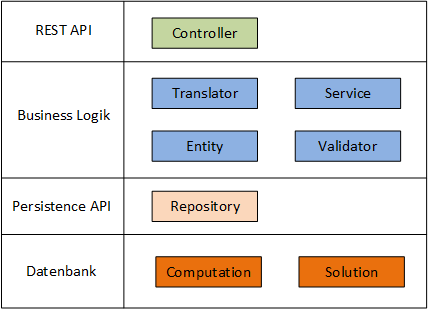
\includegraphics[scale=0.8]{images/visio/architektur_db.png}
\caption{Architekturaufbau des Systems (Eigene Darastellung)}
\label{fig:architektur}
\end{figure}
 
\FloatBarrier
\subsection{REST API}
Für die Schnittstelle wird ein REST API erstellt, welches die nötigen Funktionen bietet. Das API funktioniert nach dem De-facto-Standard (siehe \cite{wiki_restful}). Falls Fehler auftretten werden die HTTP-Statuscode verwendet, um diese an den Aufrufer weiterzugeben.

\subsection{Business Logik}
Die Business Logik besteht aus Translator, Service, Entity und Validator von den jeweiligen Problemen. Es gibt jeweils ein ProblemTranslator für die Umwandlung hin zum Algorithmus und einen SolutionTranslator für die Umwandlung vom Algorithmus zurück in das System. Der Service kann sehr generisch gehalten werden und benötigt nichts problemspezifisches. Die Entitäten sind von Problem zu Problem unterschiedlich, es muss analysiert werden, wie die Parameter am besten eingegeben werden und wie diese dann vom Algorithmus gebraucht werden. Der Validator entscheidet, ob eine Lösung gültig ist oder nicht. Wie bereits im \autoref{cat_theo_inf} erklärt, kann jedes NP-vollständige Problem kann in polynomialer Zeit validiert werden.

\subsection{Persistance API}
Die Abstraktion der Datenbank wird mittels eines Persistance APIs, welches mit der Datenbank interagiert, realisiert.

\subsection{Datenbank}
Jedes Problem hat seine eigene Ausprägung von Problem und Solution, welche abgespeichert werden müssen. Die Datenbank sollte wenn möglich eine ähnliche Flexibilität wie das Programm selber aufweisen. Die Vorgänge benötigen keine Transaktionen und sind zum grossen Teil nur Einfüge-Operationen, nur selten wird ein Einträg geändert.

\begin{landscape}
\subsection{Ablauf}
\thispagestyle{empty}
In \autoref{fig:workflow} wird der Ablauf des ganzen Vorganges und die Interaktion mit dem Nutzer und dem Verarbeitungssystem nochmals verdeutlicht.

\begin{figure}[h]
\centering
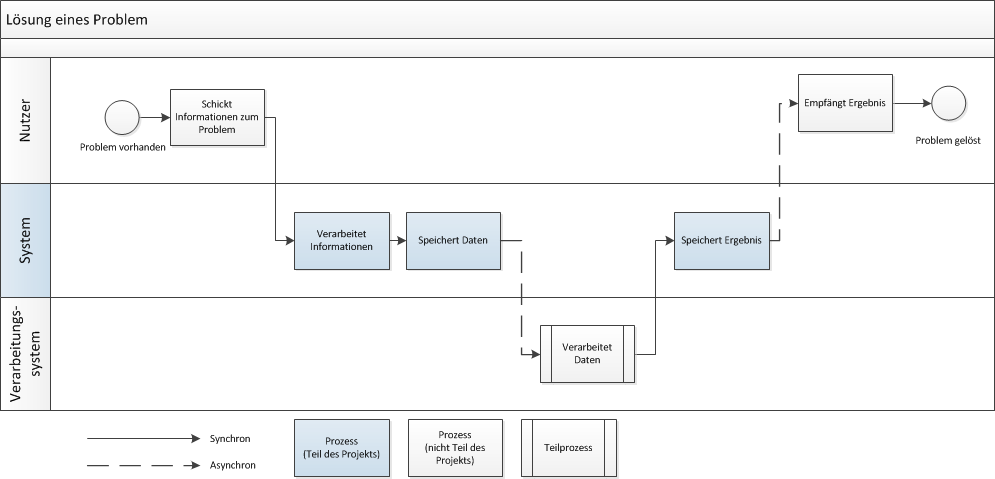
\includegraphics[scale=0.8]{images/visio/workflow.png}
\caption{Flussdiagramm des Arbeitsablaufs (Eigene Darastellung)}
\label{fig:workflow}
\end{figure}

\end{landscape}


Die \autoref{fig:sequenz_diagramm_start} zeigt das Sequenzdiagramm für den Start eines beliebigen Problems, alle Komponenten mit '{Problem}' sind spezifische Problem-Komponenten, die anderen sind generisch. Bei Speichern des Problems, wird das Problem mit dem Status 'CREATED' gespeichert. Nach dem Speichern wird über eine Solver-Komponente das Verarbeitungssystem asynchron gestartet. Das Verarbeitungssystem holt sich nun die benötigten Informationen. Der Controller lädt das Problem vom Service, dieser wiederum lädt es vom Repository und wandelt es für den Algorithmus um.

\begin{figure}[h]
\centering
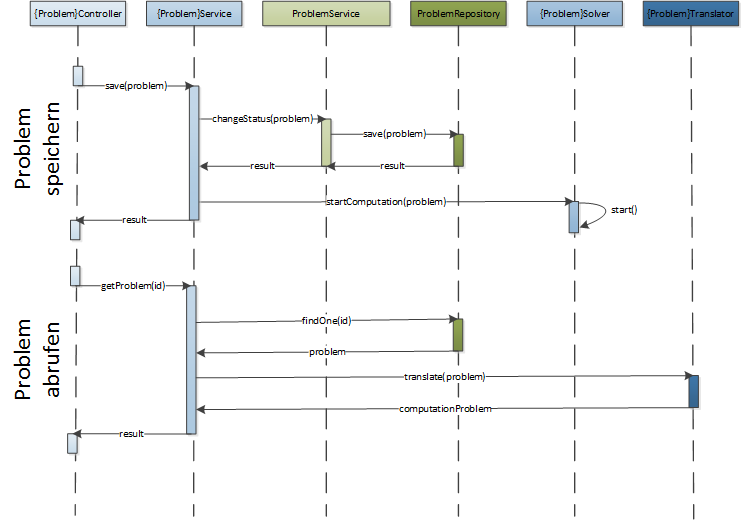
\includegraphics[scale=0.8]{images/visio/sequenz_diagramm_start.png}
\caption{Start eines belieben Problemes (Eigene Darastellung)}
\label{fig:sequenz_diagramm_start}
\end{figure}

Die \autoref{fig:sequenz_diagramm_result} zeigt das Sequenzdiagramm für das Abspeichern des Resultates eines beliebigen Problems. Bei einem Speicheraufruf wird zuerst das Problem geladen, danach wird die Lösung vom Algorithmus mit Hilfe der Eingabeparameter transferiert und vom Validator validiert. Das Resultat wird dann mit dem Ergebnis der Validierung in die Datenbank gespeichert. Wenn der Nutzer das Resultat abholt, sucht der Controller über den Service ein Endresultat für die Berechnung und liefert dieses dann dem Nutzer.

\begin{figure}[h]
\centering
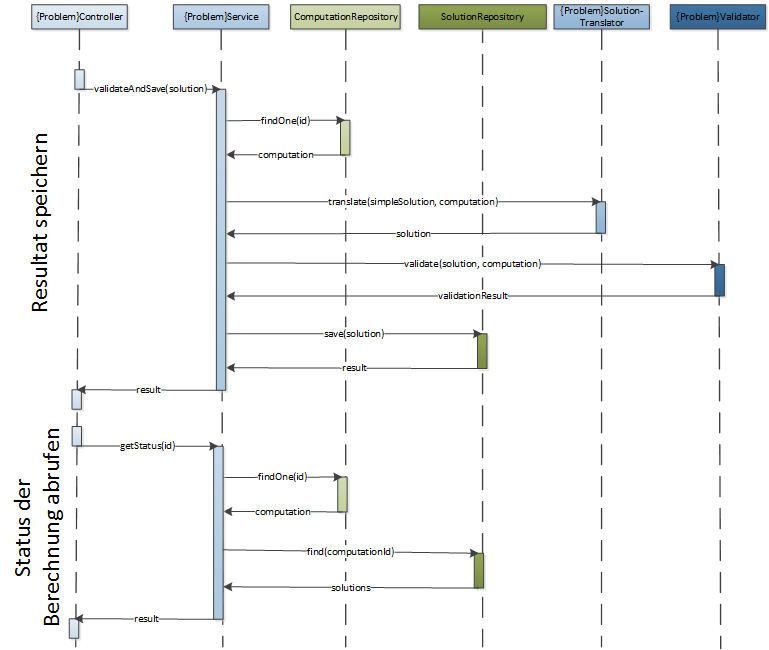
\includegraphics[scale=0.8]{images/visio/sequenz_diagramm_result.png}
\caption{Abspeichern des Resultates eines belieben Problemes (Eigene Darastellung)}
\label{fig:sequenz_diagramm_result}
\end{figure}

\section{Datenbank Varianten}\label{db_varianten}
Es gibt verschiedene Datenbanktypen und jede hat seine Vor- und Nachteile. In diesem Abschnitt werden drei verschiedenen Typen miteinander verglichen und die beste für diesen Anwendungszweck ausgewählt.

\subsection{Relationales Datenbanksystem}\label{rdbms}


\subsection{Objektorientiertes Datenbanksystem}\label{object_db}

\subsection{NoSQL Datenbanksystem}\label{no_sql_db}


\newpage
\subsection{Nutzwertanalyse}\label{architektur_nutzwertanalyse}

\subsubsection{Bewertungskriterien}\label{architektur_bewertungspunkte}

In der Nutzwertanalyse werden folgende Punkte betrachtet und nach dem angegebenen Schema bewertet und dann gewichtet. Die Kriterien sind grösstenteils aus den Softwarequalitäsmerkmalen nach \cite{iso_9126} abgeleitet.

\paragraph{Aufwand}
\begin{itemize}
	\item \textbf{Beschreibung}: Wie gross ist der geschätzte Aufwand mit dieser Methode?
	\item \textbf{Bewertung}: 1: sehr hoch, 10: sehr niedrig
	\item \textbf{Gewichtung}: 5 (Die Zeit für dieses Projekt ist beschränkt und die Entscheidung könnte zu einem Risiko werden)
\end{itemize}

\paragraph{Benutzbarkeit}
\begin{itemize}
	\item \textbf{Beschreibung}: Wie lange dauert die Einarbeitungsphase? 
	\item \textbf{Bewertung}: 1: sehr langsam, 10: sehr schnell
	\item \textbf{Gewichtung}: 4 (Umso mehr Zeit für das Erlernen investiert wird, umso weniger Zeit ist für die Implementierung vorhanden)
\end{itemize}

\paragraph{Änderbarkeit}
\begin{itemize}
	\item \textbf{Beschreibung}: Wie flexibel ist diese Variante in Bezug auf Erweiterungen/Vererbung?
	\item \textbf{Bewertung}: 1: sehr spezifisch, nicht portabel, 10: sehr flexibel
	\item \textbf{Gewichtung}: 5 (Die Anforderungen geben vor, dass das System einfach zu erweitern sein sollte)
\end{itemize}

\paragraph{Funktionalität}
\begin{itemize}
	\item \textbf{Beschreibung}: Wie gross ist der Funktionalitätsumfang?
	\item \textbf{Bewertung}: 1: sehr eingeschränkt, 10: sehr weit reichend
	\item \textbf{Gewichtung}: 1 (In der ersten Version der App wird noch nicht viel Funktionalität gebraucht)
\end{itemize}

\newpage
\subsubsection{Bewertung}\label{architektur_bewertung}


\FloatBarrier
\subsubsection{Fazit}\label{architektur_fazit}
Das Resultat der Nutzweranalyse ist eindeutig, die Entwicklung mittels Phonegap ist für dieses Projekt mit Abstand die beste Lösung. Die Methode hat noch weitere Vorteile, durch dass das der Code nur in eine App verpackt wird und er nicht in eine andere Sprache übersetzt wird, gibt es viel weniger Overhead. Zudem ist es möglich den Source auch in der App ohne Problem anzupassen, dass heisst, falls der Convert nicht mehr funktioniert, weil er zum Beispiel nicht mehr unterhalten wird, kann man torztdem noch weiterentwickeln und muss nicht zu erst ein Reverse Engineering machen.

\newpage
\section{Fazit}\label{architektur_fazit}

Obwohl die Probleme auf den ersten Blick sehr unterschiedlich sind, bleiben die groben Abläufe gleich. Somit kann einiges generalisiert werden. Ein neues Problem heisst schlussendlich neue Entities, zwei neue Translator, ein neuer Validator und ein neuer Einstiegspunkt für den Nutzer.  Controller, Services und Repositories werden generisch gehalten.



